\chapter{{Introduction}}
\label{ch_1:intro}

\begin{figure}
	\centering
	\begin{minipage}{1.1\textwidth}
		\centering
		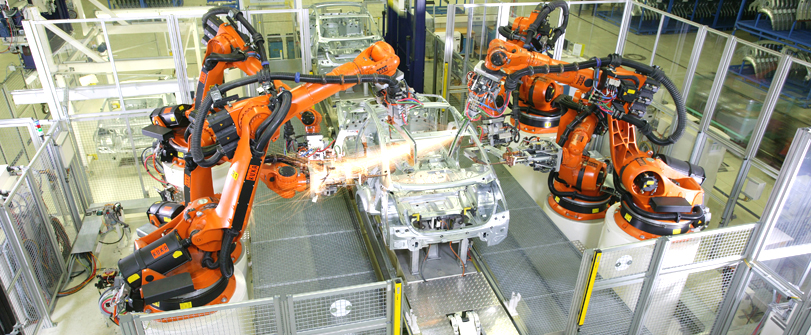
\includegraphics[height=5cm,keepaspectratio]{Chapter1/fig/factory}
		\captionof{figure}{Robotics in Factory (Source: Kuka Robot)}
		\label{fig:RF}
	\end{minipage}
\vskip 15mm
	\begin{minipage}{.5\textwidth}
		\centering
		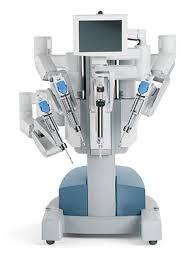
\includegraphics[height=5cm,keepaspectratio]{Chapter1/fig/healthc}
		\captionof{figure}{Health Care\\ (Source:  da Vinci Surgical System)}
		\label{fig:HC}
	\end{minipage}%
	\begin{minipage}{.5\textwidth}
		\centering
		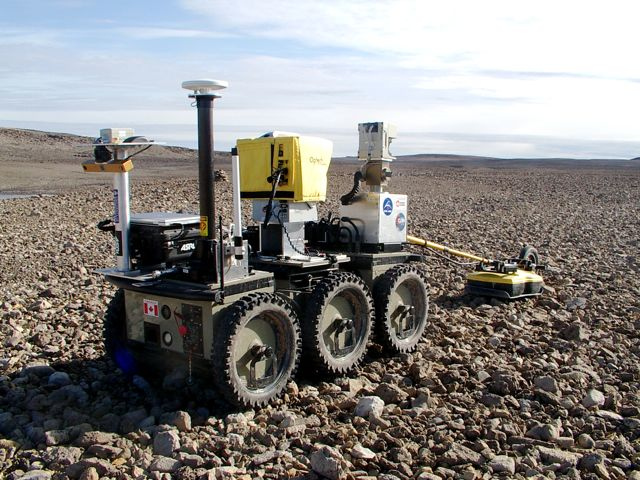
\includegraphics[width=.8\linewidth,height=5cm,keepaspectratio]{Chapter1/fig/explore}
		\captionof{figure}{Exploration and surveillance\\ Source: Autonomous Space Robotics Lab - University of Toronto}
		\label{fig:ES}
	\end{minipage}
\end{figure}
The use of robots such as robotic arm shown in Figure \ref{fig:RF} has been used in factories for a long time, basically for repetitive kind  of job. Though it started with the intention to reduce human labour, production cost, and increased productivity, with technological development  their scope has expanded beyond  manufacturing domain. Robots are now being used for health care, surveillance, exploration, etc. as illustrated in Figures \ref{fig:HC} and \ref{fig:ES}. The reduction in development cost  has resulted in introduction of robotic systems in entertainment industries and personal care as well. Robots have matured from heavy duty serial linked mechanical arms to a more presentable form such as ASIMO ( Figure \ref{fig:HAsimo}) by Honda and Aibo by Sony  ( Figure \ref{fig:SA}).  
\begin{figure}
	\centering
	\begin{minipage}{.5\textwidth}
		\centering
		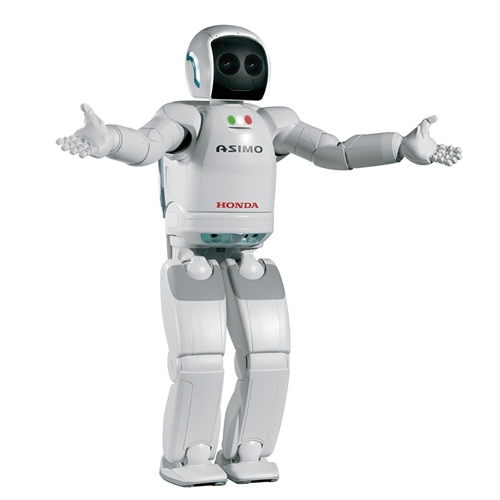
\includegraphics[height=5cm,keepaspectratio]{Chapter1/fig/Honda-Asimo}
		\captionof{figure}{Honda Asimo \\Source:http://asimo.honda.com}
		\label{fig:HAsimo}
	\end{minipage}%
	\begin{minipage}{.5\textwidth}
		\centering
		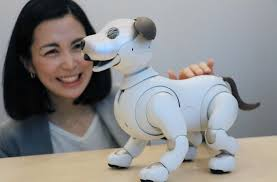
\includegraphics[width=.8\linewidth,height=5cm,keepaspectratio]{Chapter1/fig/aibo}
		\captionof{figure}{Sony Abio\\ Source: https://us.aibo.com/}
		\label{fig:SA}
	\end{minipage}
\end{figure}

 In areas where human access is not preferred or restricted  due to risk of life or inhospitable environmental conditions as in chemical, space or nuclear industries, robotic systems have gained huge popularity in providing services as surveillance, rescue, exploration and remote maintenance.  Research in teleoperated and autonomous mobile robotics has been fuelled largely by these  requirement. Teleoperated mobile robots are suitable for these applications  as the workspace required to be covered is very large, and it is essential to maintain  physical separation between the robot and its control station. Moreover, the remote environment is in general unknown. 
 
 The present research too was motivated by a similar requirement for in-situ measurement of the ionizing radiation and  neutron field, inside the vault and cave areas of   K-130,  K-500  and Medical Cyclotron operational at VECC, Kolkata, West Bengal. Cyclotrons are used to accelerate  charged particles to high energies. These are required for experiments in nuclear physics and nuclear medicine. The particles are accelerated to high energy using a high frequency alternating voltage, which is applied between two hollow "D"-shaped sheet metal electrodes called "Dees" inside a vacuum chamber. The area surrounding the Dee is called the vault.  The cave is the area where beam line (beam of  accelerated charged particles) is available for experimentation. Radiation mapping of these areas is a  mandatory requirement for getting safety clearance from regulators during  commissioning of new units and at regular intervals during operational life of the cyclotron facility.   Though, there are radiation detectors placed at different locations in these areas they can only measure radiation levels at discrete locations, but can not provide the 3-D radiation  map. The advantage of having a  radiation map is that it  provide detailed  input to health physicist  of the dose a person may receive and accordingly plan emergency  operations. These maps also provide the plant operators with the location of radiation leakage and accordingly tune the system to improve its efficiency.

The challenge faced for in-situ inspection during operation of cyclotron is that the interaction  between  an  accelerated  beam   of  charged  particles  and  the  target  produce Bremsstraghlung and characteristic x-rays, prompt $\gamma$-rays, neutrons and delayed radiation ($\beta $ and $\gamma$) this makes human presence unacceptable.  A teleoperated mobile robot with wireless communication link is the obvious solution. This thesis discusses the design, analysis and development of a prototype robot  to carry out in-situ measurement and mapping of radiation level.
% \setcounter{secnumdepth}{4} 
\chapter{Literature Review}
\label{c2_LitRev}

In this chapter, we  discuss some of the important works published pertaining to the scope of this thesis. Few of the techniques and methods published in these literatures are directly used. The section on \textit{Special Purpose Robots} lists literature which were reviewed to arrive at the overall design of the mobile robot developed in this research.
 The dynamic analysis of the mobile platform was based on the works cited in section\textit{ Mathamatical Modeling}. 
 The literature discussed in \textit{Path Tacking } helped to arrive at the "human model" proposed in this thesis for simulation of teleoperation. 
 The section on \textit{Tele-operation} discusses literature in a much broader sense; such as force feedback, haptic interface  design, etc., than what was adapted in this thesis. 
 This was done for completeness of the subject. 
 Last section on \textit{Predictive Display}, though a part of human interface for tele-operation is discussed separately because it forms one of the major components of the tele-operation system network designed  for the mobile robot  presented in this thesis.   
\section{ Special Purpose Robots}
This section reviews some of the special purpose  robots built for various typical applications. 
Design and fabrication of a low cost, solar powered mobile robot for  scientific missions on the Antarctic plateau was presented by Ray  \cite{ray2005design}. Honeycomb-glass-fibre composite was used to provide high strength and low weight. Ohno, et al. \cite{ohno2011robotic}   developed a robotic  vehicle shown in Figure \ref{fig:fukuRobot} for measuring the radiation in the Fukushima Daiichi Nuclear Power Plant. A survey of different types of climbing robots for non-destructive testing of pressure vessel is given by \cite{luk2006tele}, such as NERO III shown in Figure \ref{fig:nero3}.  Briones \cite{briones1994wall} presents a vacuum cup based wall climbing robot for inspection of  nuclear power plants. Galt \cite{galt1997tele} has developed eight-legged teleoperated mobile robot for the use in nuclear industry. Development of a magnetic-wheel based mobile robot for painting of ship is discussed by Cho \cite{cho2013study}. Compliant link based mobile robot was designed and tested by Borenstein\cite{borenstein1995control}, in which the author claims that due to its unique design, better dead-reckoning accuracy was achieved compared to other contemporary designs. This vehicle has two independent drive units or "trucks" that are free to rotate about a vertical shaft connected to the vehicle body. Each truck comprises two drive motors on a common axes and forms a differential drive system. Mechanical compliance was implemented by means of a linear bearing that allows relative motion between the front and rear truck. Other literature giving details of  mobile robots based on   differential wheel, traction belt and omnidirectional wheel are given in the introductory part of Chapter \ref{ch_3:Design}.
 \begin{figure}
	\centering
	\begin{minipage}{.5\textwidth}
		\centering
		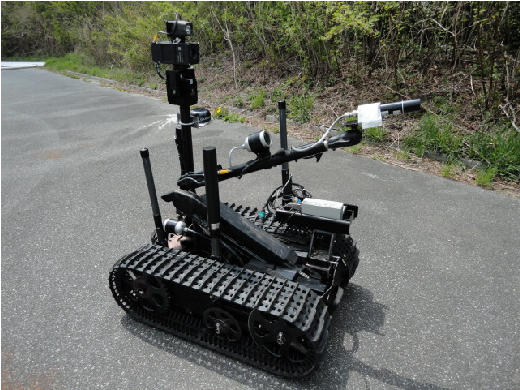
\includegraphics[height=5cm,keepaspectratio]{Chapter2/fig/FukusimaRobot}
		\captionof{figure}{Robot for Fukushima Daiichi \\  Source:  Ohno, et al  \cite{ohno2011robotic} }
		\label{fig:fukuRobot}
	\end{minipage}%
	\begin{minipage}{.5\textwidth}
		\centering
		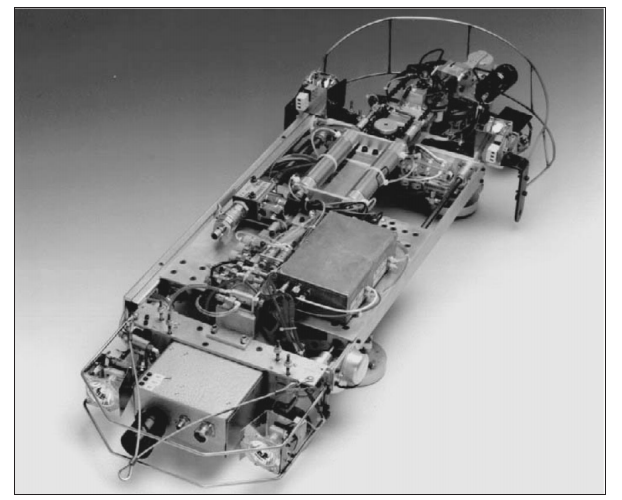
\includegraphics[width=1\linewidth,height=5cm,keepaspectratio]{Chapter2/fig/nero3}
		\captionof{figure}{NERO III \\ Source: Luk et al \cite{luk2006tele}}
		\label{fig:nero3}
	\end{minipage}
\end{figure}

   
\section{Mathematical Modeling}
A very comprehensive list of Wheeled Mobile Robots (WMR) using different wheel configuration is given by Muir and Neuman \cite{muir1987kinematic}. In the paper, kinematic equations of conventional, omnidirectional and ball wheels were presented. The kinematics of the WMR was derived by combining the kinematic information of   individual wheel. Detection of wheel slip based on  error in the least square solution was also discussed. Similar issues were addressed by Alexander in \cite{alexander1989kinematics}. The major difference is that he uses physical friction model in the analysis of over actuated systems where rolling constrains are not satisfied. A seminal work by Champion \cite{campion1996structural} gives the structural classification of wheeled mobile robots based on the \textit{degree of mobility}, $\delta_m$, and \textit{degree of steeribility}, $\delta_s$. It was based on the number of conventional fixed wheels and  conventional centered orientable wheels. According to them any WMR fall in one of the 5 categories given by $(\delta_m,\delta_s)\rightarrow(3,0),(2,1),(1,1),(1,2)$. 
The configuration and posture kinematic models of each type was derived. Based on  dynamic model, the minimal number of actuators required for full maneuverability of each type was presented. Kinematic analysis of omi-directional over-actuated mobile robot  was presented in \cite{yi2002kinematics}. Two different methods for forward kinematics was also discussed along with  singularity analysis. Actuator switching scheme based on load distribution to avoid singularity was also presented. 

Dynamic modeling of mobile manipulator can be categorized as: force based ,i.e, the Newtaon-Eular (NE) formulation and  energy based as in Eular-Lagrange (EL) equations. Hoostmans \cite{hootsmans1992motion} used NE method to arrive at  the dynamic model of a mobile manipulator that has two links mounted on a mobile platform. Chung \cite{chung1998interaction} used EL method to arrive at the equations of motion for a mobile manipulator. Geometric mechanics was used to adapt Luh and walker \cite{luh1980line} algorithm  by Boyer and Ali \cite{boyer2011recursive} to apply recursive inverse dynamics formulation to wheeled systems.   

Orthogonal compliment method utilizes the advantage of NE and EL approach to derive the equations of motion of  a multibody  system.  It uses the fact that the motion can take place only in the null space of the constrains inducing matrix $A$ defined as $Ax=0$, where $x$ is a vector of independent co-ordinates. The orthogonal compliment of the constraint inducing matrix $A$ is used to eliminate the non-working constraint  forces  and moments from the equations of motion.  Angeles and Lee \cite{angeles1988formulation} used the natural orthogonal compliment method to derive the equations of motion for holonomic mechanical systems. In this,  orthogonal compliment was derived from the velocity constraints naturally, hence the name. This was  used by Angeles \cite{angeles2013fundamentals} and Saha in \cite{saha1989kinematics},\cite{saha1991dynamics} to derive the equations of motion for a WMR. 

\section{Path Tracking}
Path tracing algorithm for the control of a mobile robot is used to arrive at the mathematical model of a human operator for simulation of tele-operation loop, as done in chapter 6. Geometry based path tracking algorithms are most intuitive and hence suitable for the present application. The major algorithms in this  category reported in the literatures are \textit{pure pursuit} \cite{coulter1992implementation}, \textit{follow the carrot} \cite{barton2001controller}, \textit{vector pursuit} \cite{wit2004autonomous}, and \textit{follow the past} \cite{hellstrom2006follow}. In pure-pursuit \cite{coulter1992implementation}, the steer angle of the robot is set so that the robot moves in circle to reach a \textit{ goal point} on the desired path. The goal point is based on the "Look Ahead Distance", which is practically the maximum distance one can see from the current vehicle position. The detailed discussion is given in Chapter \ref{c6_simulation}.  Corrective action was based on  position error of the vehicle, where orientation error was not taken into account explicitly. 

In case of "Follow the Carrot" method \cite{barton2001controller},  the steering angle is set proportional to the \textit{orientation error} defined in Figure \ref{fig:FollowCarrot}. The orientation error is defined as the difference between the current orientation of the vehicle and the orientation required from the present position of the vehicle to reach the goal point on the referance path.  The proportionality constant is decided based on trial and error.

 \begin{figure}
	\centering
	\begin{minipage}{.5\textwidth}
		\centering
		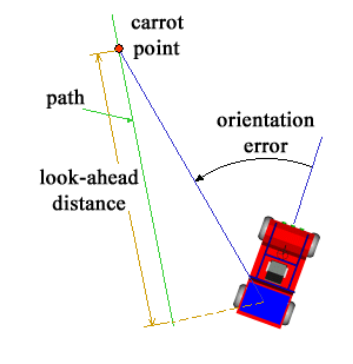
\includegraphics[height=5cm,keepaspectratio]{Chapter2/fig/FollowTheCarrot}
		\captionof{figure}{Follow the carrot}
		\label{fig:FollowCarrot}
	\end{minipage}%
	\begin{minipage}{.5\textwidth}
		\centering
		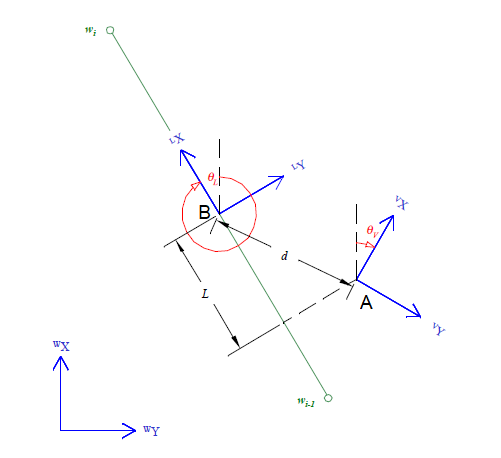
\includegraphics[width=1\linewidth,height=5cm,keepaspectratio]{Chapter2/fig/VectorPursuit}
		\captionof{figure}{Vector pursuit}
		\label{fig:VectorPursuit}
	\end{minipage}
\end{figure}
 The two previous geometric path tracking techniques  generate steering commands based upon the goal point on the reference trajectory to be traced. 
 %The requirement of vehicle posture control for accurate trajectory following remains unsatisfied.  
 Wit in \cite{wit2004autonomous} suggested a strategy to uses the path orientation and curvature  known at the goal point to improved path tracking,  such that the vehicle arrived at the goal point  with the correct orientation and curvature. Wit used Screw theory to find the error between the screw at the current location, point $A$  and the required screw at the goal position, Point $b$ as shown in Figure \ref{fig:VectorPursuit}. Control is then generated proportional to this error.

Hellstrom \cite{hellstrom2006follow} has proposed an algorithm which uses the knowledge of previously recorded steer angle, associated with  the path traced earlier. In this algorithm, the steer angle of the vehicle is set based on the orientation error, position error and the past recorded steer angle. A recent survey by Paden \cite{paden2016survey} provides extensive review of other control strategies for path tracking of autonomous unmanned vehicles such as those based on Lyapunov method, Model Predictive Controller, adaptive control, etc. 


   
\section{Tele-operation}
Tele-operation deals with  connecton of a   human operator with the robot in order to reproduce human action at distance. Tele-operation is in general bidirectional or bilateral as the human needs to have a feedback in order to understand the results of his action and to perceive the remote environment. It started with its use in nuclear and space industries \cite{martin1985teleoperated,vertut1986teleoperations}, but now it is used in underwater exploration, surgery, live-power line maintenance, mining, etc. All characterized by reducing the risk to human operators. The two major related research areas are the "human interface" and "control" design.
\subsection{Human interface}

Human interface is a means through which the operator interacts with the remote robot by perceiving the remote environment and sending commands accordingly. Thus, the human interface has two important purpose: one to excite the human senses to show the action of the executed task and to process the human command properly to execute it at the remote end.  Force and haptic feedback of remote environment drastically improves operator's performance. Hence a serial link haptic device PHANTOM \cite{massie1994phantom} was developed at MIT during 1994 to provide 3-DOF force feedback  for touch feedback purpose. DELTA Haptice Device described in \cite{grange2001overview} provides 6-DOF force feedback with moderate force. Clover \cite{clover1997dynamic} has reported  the use of off-the-shelf serial industrial robots for haptic realization of tasks requiring a large workspace and high force capability. Customized 10-DOF  haptic device was reported  for similar purpose in \cite{ueberle2004vishard10}. Design  of a 6-DOF parallel mechanism for force feedback is discussed in \cite{yoon2001design}.

Another major form of human interface is the visual feedback. The main challenge is to provide depth perception of remote environment. Most stereoscopic systems used in telerobotics are based on shutter glasses \cite{aracil1997telerobotic,matthies1992stereo}, head-mounted displays \cite{matthies1992stereo} or polarized images \cite{hirzinger1994robots}. Systems based on shutter glasses hide user's eyes alternately in synchronization to screen refreshment, which projects images for left and right eye alternately. A second type of interfaces is based on polarized images. The user is also required to wear glasses that filter the left and right images. The third type of interface is  the head mounted display such as "Google cardboard",  especially designed to immerse users into virtual environments where the left and right images are projected on each eye using two separate screens or split screens.

\subsection{Control}
Control of a tele-operetion system deals with two issues, \textit{transparency} and \textit{stability}. Transparency deals with what information is to be exchanged between the remote and local station so that the operator can have a natural feel of the remote environment. A position-position architecture is suggested by  Goertz \cite{goertz1961anl}, where  master position is passed as a command to the slave servo (position) controller, and slave position is returned to the master as a position command. A position-force architecture has been proposed by Flatau \cite{flatau1977sm} in which the master sends the position to the slave and the slave sends back the force felt by it in the remote environment. A general 4-channel architecture been suggested by Lawrence \cite{lawrence1993stability}, and transparency has been defined  as a measure of performance in teleoperation and evaluated for different architectures.
 
An excellent survey article on control of bilateral teleoperation was given by Hokayem and Spong \cite{hokayem2006bilateral}. Few of these are briefly presented here. A teleoperation system, comprised of a master and slave with their corresponding controllers, residing between the human operator and the environment,   can be modeled as a two port network. Passivity based design of stabilizing control using  wave-variable concept and scattering theory has been proposed by Anderson and Spong \cite{anderson1989bilateral}, Rebelo \cite{rebelo2015time} and Anderson and Slotin \cite{niemeyer1991stable}.   Port-Hamiltonian  based approach was used in \cite{stramigioli2010novel,stramigioli2005sampled}. Design of controller for time delayed systems  based on back-stepping method in combination with partial differential heat  equation was studied by  Kristic \cite{krstic2009delay}. 



\section{Predictive Display}
Delays are inherent in teleoperation over wireless network. Practically, much of the delay is due to relay stations and limited  bandwidth of the network.  As little as a half second delay in the visual feedback significantly reduces human performance \cite{chen2007human}. The operator tends to adopt an inefficient "move then wait and see" policy in order to complete the task.

    To overcome performance deterioration of the operator due to time delay in visual feedback, two approaches have been reported in the literature, namely, \textit{supervisory control or tele-assistance  } and \textit{predictive display}. In \textit{supervisory control} \cite{sheridan1986human,pook1994teleassistance,jagersand1995visual} the robot is partly guided by operator by giving the robot intermittent commands to achieve the goal. The drawback of such system is that operator looses direct contact with the task.
    In  predictive display systems, a natural and widely used techniques, synthesised view of the remote environment is displayed to the operator based on his movements. It has been used for space teleoperation as early as in 1993, which was reported by Sherdan \cite{sheridan1993space}, Bejczy \cite{bejczy1990predictive} and Kim \cite{kim1993demonstration}. Whereas the above two used a-prior modeling and  calibration of remote environment, Jagersand \cite{jagersand1999image} used delayed visual feedback and operator control signal to build predicated image which was presented to the operator. The system was implemented with a fixed remote environment with a manipulator arm with  two wall mounted cameras. An estimation function was proposed 
    $I_i \approx \phi_k(x_i), i \in {1,..k}$, that approximated each image  $I_i$ seen so far on the trajectory, i.e, ${x_1, x_2 .....x_k}$. Un-calibrated monocular camera mounted on manipulator (eye-in-hand) based image predication method was discussed   by Yeres \cite{yerex2003predictive} and Deng \cite{deng2003predictive}. Multiple sensors based dense 3-D  map of a remote scene was reported by Kelly \cite{kelly2011real} and \cite{burkert2004photorealistic}. While Kelly used fusion of  lidar and  camera,  Burkert used stereo cameras. Hu \cite{hu2015line} has used SLAM based Predictive Dispalay  (PD) system for telemanipulation of a mobile robot. In his approach, texture and geometry of the remote site was transmitted instead of  video stream. This, the author, claims reduces bandwidth utilization.
    \section{Summary}
    Different literatures relevant to the topic addressed in this research were presented. Each topic is a separate area of research in its self.  There are many more literatures in each topic which could be of great interest but was been skipped due to space constraints.  



\section{Literature Survey}
\label{sec_LitRev}
In this section r, we  discuss some of the important works published pertaining to the scope of this thesis. Few of the techniques and methods published in these literatures are directly used. The section on \textit{Special Purpose Robots} lists literature which were reviewed to arrive at the overall design of the mobile robot developed in this research.
The dynamic analysis of the mobile platform was based on the works cited in section\textit{ Mathamatical Modeling}. 
The literature discussed in \textit{Path Tacking } helped to arrive at the "human model" proposed in this thesis for simulation of teleoperation. 
The section on \textit{Tele-operation} discusses literature in a much broader sense; such as force feedback, haptic interface  design, etc., than what was adapted in this thesis. 
This was done for completeness of the subject. 
Last section on \textit{Predictive Display}, though a part of human interface for tele-operation is discussed separately because it forms one of the major components of the tele-operation system network designed  for the mobile robot  presented in this thesis.   
\subsection{ Special Purpose Robots}
This section reviews some of the special purpose  robots built for various typical applications. 
Design and fabrication of a low cost, solar powered mobile robot for  scientific missions on the Antarctic plateau was presented by Ray  \cite{ray2005design}. Honeycomb-glass-fibre composite was used to provide high strength and low weight. Ohno, et al. \cite{ohno2011robotic}   developed a robotic  vehicle shown in Figure \ref{fig:fukuRobot} for measuring the radiation in the Fukushima Daiichi Nuclear Power Plant. A survey of different types of climbing robots for non-destructive testing of pressure vessel is given by \cite{luk2006tele}, such as NERO III shown in Figure \ref{fig:nero3}.  Briones \cite{briones1994wall} presents a vacuum cup based wall climbing robot for inspection of  nuclear power plants. Galt \cite{galt1997tele} has developed eight-legged teleoperated mobile robot for the use in nuclear industry. Development of a magnetic-wheel based mobile robot for painting of ship is discussed by Cho \cite{cho2013study}. Compliant link based mobile robot was designed and tested by Borenstein\cite{borenstein1995control}, in which the author claims that due to its unique design, better dead-reckoning accuracy was achieved compared to other contemporary designs. This vehicle has two independent drive units or "trucks" that are free to rotate about a vertical shaft connected to the vehicle body. Each truck comprises two drive motors on a common axes and forms a differential drive system. Mechanical compliance was implemented by means of a linear bearing that allows relative motion between the front and rear truck. Other literature giving details of  mobile robots based on   differential wheel, traction belt and omnidirectional wheel are given in the introductory part of Chapter \ref{ch_3:Design}.
\begin{figure}
	\centering
	\begin{minipage}{.5\textwidth}
		\centering
		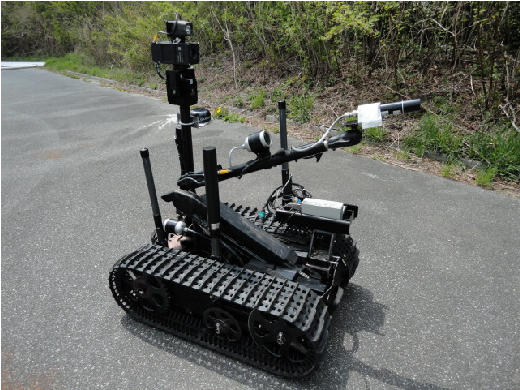
\includegraphics[height=5cm,keepaspectratio]{Chapter2/fig/FukusimaRobot}
		\captionof{figure}{Robot for Fukushima Daiichi \\  Source:  Ohno, et al  \cite{ohno2011robotic} }
		\label{fig:fukuRobot}
	\end{minipage}%
	\begin{minipage}{.5\textwidth}
		\centering
		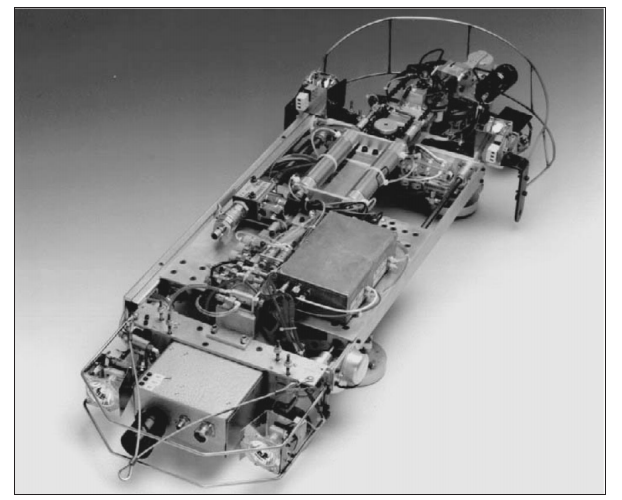
\includegraphics[width=1\linewidth,height=5cm,keepaspectratio]{Chapter2/fig/nero3}
		\captionof{figure}{NERO III \\ Source: Luk et al \cite{luk2006tele}}
		\label{fig:nero3}
	\end{minipage}
\end{figure}


\subsection{Mathematical Modeling}
A very comprehensive list of Wheeled Mobile Robots (WMR) using different wheel configuration is given by Muir and Neuman \cite{muir1987kinematic}. In the paper, kinematic equations of conventional, omnidirectional and ball wheels were presented. The kinematics of the WMR was derived by combining the kinematic information of   individual wheel. Detection of wheel slip based on  error in the least square solution was also discussed. Similar issues were addressed by Alexander in \cite{alexander1989kinematics}. The major difference is that he uses physical friction model in the analysis of over actuated systems where rolling constrains are not satisfied. A seminal work by Champion \cite{campion1996structural} gives the structural classification of wheeled mobile robots based on the \textit{degree of mobility}, $\delta_m$, and \textit{degree of steeribility}, $\delta_s$. It was based on the number of conventional fixed wheels and  conventional centered orientable wheels. According to them any WMR fall in one of the 5 categories given by $(\delta_m,\delta_s)\rightarrow(3,0),(2,1),(1,1),(1,2)$. 
The configuration and posture kinematic models of each type was derived. Based on  dynamic model, the minimal number of actuators required for full maneuverability of each type was presented. Kinematic analysis of omi-directional over-actuated mobile robot  was presented in \cite{yi2002kinematics}. Two different methods for forward kinematics was also discussed along with  singularity analysis. Actuator switching scheme based on load distribution to avoid singularity was also presented. 

Dynamic modeling of mobile manipulator can be categorized as: force based ,i.e, the Newton -Euler (NE) formulation and  energy based as in Eular-Lagrange (EL) equations. Hoostmans \cite{hootsmans1992motion} used NE method to arrive at  the dynamic model of a mobile manipulator that has two links mounted on a mobile platform. Chung \cite{chung1998interaction} used EL method to arrive at the equations of motion for a mobile manipulator. Geometric mechanics was used to adapt Luh and walker \cite{luh1980line} algorithm  by Boyer and Ali \cite{boyer2011recursive} to apply recursive inverse dynamics formulation to wheeled systems.   

Orthogonal compliment method utilizes the advantage of NE and EL approach to derive the equations of motion of  a multibody  system.  It uses the fact that the motion can take place only in the null space of the constrains inducing matrix $A$ defined as $Ax=0$, where $x$ is a vector of independent co-ordinates. The orthogonal compliment of the constraint inducing matrix $A$ is used to eliminate the non-working constraint  forces  and moments from the equations of motion.  Angeles and Lee \cite{angeles1988formulation} used the natural orthogonal compliment method to derive the equations of motion for holonomic mechanical systems. In this,  orthogonal compliment was derived from the velocity constraints naturally, hence the name. This was  used by Angeles \cite{angeles2013fundamentals} and Saha in \cite{saha1989kinematics},\cite{saha1991dynamics} to derive the equations of motion for a WMR. 
\subsection{Stability of Mobile Manipulator}
Stability of mobile manipulators has been studied by both the vehicular community and the robotics community. The vehicular community has focused on characterizing the lateral rollover of the vehicle as in  \cite{buchele1990computer,jones1990engineering}. The robotic community has discussed problem from motion planing of manipulator and has come up with different stability margins. Dubowsky \cite{dubowsky1989planning} has studied the motion planning of mobile manipulator for stationary platform. The criterion for stability is that the support point should not loose ground contact. McGhee \cite{mcghee1968stability} proposed as shortest distance between the Center of Gravity  and the edge of the support polygon projected on a horizontal plane. \textit{Zero moment point} (ZMP) was developed to study the stability of biped mechanism by  Vukobratovic et al. \cite{vukobratovic1969contribution,vukobratovic2012biped}. It was later adapted by Ollero \cite{ollero1995stability} , Hung et al. \cite{huang1995manipulator,huang1994stability}  and Sugano \cite{sugano1993stability} to examine the stability of mobile manipulators. Furuno \cite{furuno2003trajectory} propose the method for planning the trajectory of the nonholonomic mobile manipulator from its end-effector's path  considering the dynamic stability. Then ZMP criterion proposed is used as an index for the system stability. Messuri et al. \cite{messuri1985automatic} proposed the stability measure called '\textit{Energy Stability Margin}'.The uses  minimum work required to tipover the legged vehicle, a measure which is sensitive to c.g. height. Ghasempoor and Sepehri \cite{ghasempoor1995measure}  extend the method of Messuri by including include external and inertial loads.   \textit{ Force-angle stability} measure which is a simple graphical method was proposed by Papadopoulo \cite{papadopoulos1996new,papadopoulos2000force}. The method is applicable to system subjected to inertial and external forces, operating over even and uneven terrains. 
\subsection{Path Tracking}
Path tracing algorithm for the control of a mobile robot is used to arrive at the mathematical model of a human operator for simulation of tele-operation loop, as done in chapter 6. Geometry based path tracking algorithms are most intuitive and hence suitable for the present application. The major algorithms in this  category reported in the literatures are \textit{pure pursuit} \cite{coulter1992implementation}, \textit{follow the carrot} \cite{barton2001controller}, \textit{vector pursuit} \cite{wit2004autonomous}, and \textit{follow the past} \cite{hellstrom2006follow}. In pure-pursuit \cite{coulter1992implementation}, the steer angle of the robot is set so that the robot moves in circle to reach a \textit{ goal point} on the desired path. The goal point is based on the "Look Ahead Distance", which is practically the maximum distance one can see from the current vehicle position. The detailed discussion is given in Chapter \ref{c6_simulation}.  Corrective action was based on  position error of the vehicle, where orientation error was not taken into account explicitly. 

In case of "Follow the Carrot" method \cite{barton2001controller},  the steering angle is set proportional to the \textit{orientation error} defined in Figure \ref{fig:FollowCarrot}. The orientation error is defined as the difference between the current orientation of the vehicle and the orientation required from the present position of the vehicle to reach the goal point on the referance path.  The proportionality constant is decided based on trial and error.

\begin{figure}
	\centering
	\begin{minipage}{.5\textwidth}
		\centering
		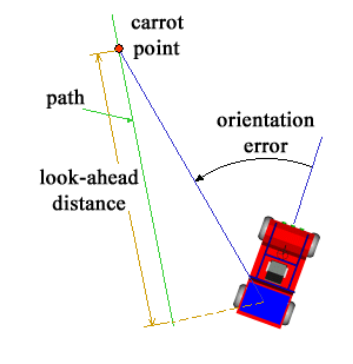
\includegraphics[height=5cm,keepaspectratio]{Chapter2/fig/FollowTheCarrot}
		\captionof{figure}{Follow the carrot}
		\label{fig:FollowCarrot}
	\end{minipage}%
	\begin{minipage}{.5\textwidth}
		\centering
		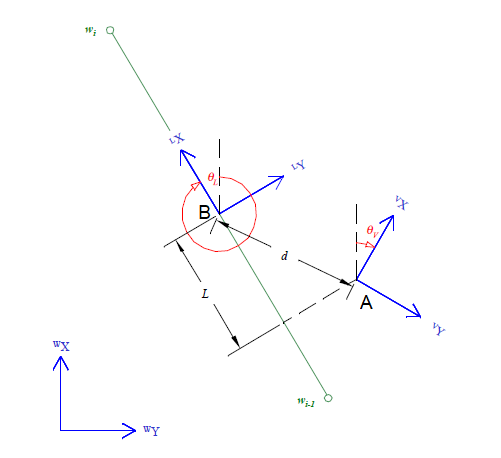
\includegraphics[width=1\linewidth,height=5cm,keepaspectratio]{Chapter2/fig/VectorPursuit}
		\captionof{figure}{Vector pursuit}
		\label{fig:VectorPursuit}
	\end{minipage}
\end{figure}
The two previous geometric path tracking techniques  generate steering commands based upon the goal point on the reference trajectory to be traced. 
%The requirement of vehicle posture control for accurate trajectory following remains unsatisfied.  
Wit in \cite{wit2004autonomous} suggested a strategy to uses the path orientation and curvature  known at the goal point to improved path tracking,  such that the vehicle arrived at the goal point  with the correct orientation and curvature. Wit used Screw theory to find the error between the screw at the current location, point $A$  and the required screw at the goal position, Point $b$ as shown in Figure \ref{fig:VectorPursuit}. Control is then generated proportional to this error.

Hellstrom \cite{hellstrom2006follow} has proposed an algorithm which uses the knowledge of previously recorded steer angle, associated with  the path traced earlier. In this algorithm, the steer angle of the vehicle is set based on the orientation error, position error and the past recorded steer angle. A recent survey by Paden \cite{paden2016survey} provides extensive review of other control strategies for path tracking of autonomous unmanned vehicles such as those based on Lyapunov method, Model Predictive Controller, adaptive control, etc. 


\subsection{Obstacle avoidance and path planing}

\textbf{The robotic system developed is not an autonomous mobile robot as it is controlled from the remote station by an operator. In future it might be required to provide autonomous navigation to the mobile robot. Autonomous navigation has two impotent ingredients; path planing and obstacle avoidance. In this section we will look at the available algorithms and techniques that has been proposed by different authors in the field of autonomous navigation. } 

\textbf{The purpose of obstacle avoidance algorithms is to avoid collisions with obstacles.Obstacle avoidance algorithms deals with moving the robot based on the feedback
information from its sensors. Virtual Force Field (VFF) method was proposed by Bornstein \cite{borenstein1989real} for  real-time obstacle avoidance for a mobile robot. In this method the robot work space is grids and each grid is given a value based on the chance of  the obstacle being  located in the cell. the amount of repulsive force acting on the robot is inversely proportional to the distance between the occupied cell and the robot. Borenstein and Koren \cite{borenstein1991vector} in this method polar histogram is around the robot.The sectors presented in the polar histogram show the \textit{polar obstacle density}. The direction of the robot is computed by choosing the sector with least concentration of obstacles. The VFH+ suggested in \cite{ulrich1998vfh+} improves upon the VFH  by introducing  \textit{threshold hysteresis} to improve the shape of the trajectory, and the use of a cost function. The Dynamic Window Approach (DWA) \cite{brock1999high} is another method for reactive obstacle avoidance dealing with the kinematical and dynamic constraints of the vehicle in contrast to VFF and VFH methods. Real-Time Obstacle Avoidance  using artificial potential field method has been used in \cite{khatib1986real},\cite{tang2010novel},\cite{park2001obstacle}. Obstacle avoidance in highly dense and troublesome environment using Nearness Diagram (ND) is presented in \cite{minguez2004nearness}. This method uses\textit{divide and conquer} approach splitting the environment into sectors to represent the location of obstacles. }

\textbf{Some of the major path planning methods are the well know \textbf{A*} method, Visibility Graph, Artificial potential method and  Voronoi diagram method \cite{garrido2006voronoi}. In the A* \cite{latombe2012robot} is a heuristic method in which the space is divide into grids, a collision  free path is found by joining the adjacent free cells. A modified version of A* is presented in \cite{duchovn2014path}.
Visibility graph method presented in \cite{nilsson1969mobile}, in which the obstacles are represented as convex polygon, a line is joined from between the vertices of the polygon with out passing through it. An algorithm search the path by joining these lines from the robot current location to the goal position.
The Voronoi diagram \cite{latombe2012robot, bhattacharya2008roadmap, takahashi1989motion} consists of arcs (lines) which are equidistant from the two nearest obstacles. The obstacles in the Voronoi diagram are presented as polygons.
The maximized clearance between the Voronoi arc segments and the polygons helps the robot maintain safe distance away from the obstacles.  }
\subsection{Tele-operation}
Tele-operation deals with  connecton of a   human operator with the robot in order to reproduce human action at distance. Tele-operation is in general bidirectional or bilateral as the human needs to have a feedback in order to understand the results of his action and to perceive the remote environment. It started with its use in nuclear and space industries \cite{martin1985teleoperated,vertut1986teleoperations}, but now it is used in underwater exploration, surgery, live-power line maintenance, mining, etc. All characterized by reducing the risk to human operators. The two major related research areas are the "human interface" and "control" design.
\subsubsection{Human interface}

Human interface is a means through which the operator interacts with the remote robot by perceiving the remote environment and sending commands accordingly. Thus, the human interface has two important purpose: one to excite the human senses to show the action of the executed task and to process the human command properly to execute it at the remote end.  Force and haptic feedback of remote environment drastically improves operator's performance. Hence a serial link haptic device PHANTOM \cite{massie1994phantom} was developed at MIT during 1994 to provide 3-DOF force feedback  for touch feedback purpose. DELTA Haptice Device described in \cite{grange2001overview} provides 6-DOF force feedback with moderate force. Clover \cite{clover1997dynamic} has reported  the use of off-the-shelf serial industrial robots for haptic realization of tasks requiring a large workspace and high force capability. Customized 10-DOF  haptic device was reported  for similar purpose in \cite{ueberle2004vishard10}. Design  of a 6-DOF parallel mechanism for force feedback is discussed in \cite{yoon2001design}.

Another major form of human interface is the visual feedback. The main challenge is to provide depth perception of remote environment. Most stereoscopic systems used in telerobotics are based on shutter glasses \cite{aracil1997telerobotic,matthies1992stereo}, head-mounted displays \cite{matthies1992stereo} or polarized images \cite{hirzinger1994robots}. Systems based on shutter glasses hide user's eyes alternately in synchronization to screen refreshment, which projects images for left and right eye alternately. A second type of interfaces is based on polarized images. The user is also required to wear glasses that filter the left and right images. The third type of interface is  the head mounted display such as "Google cardboard",  especially designed to immerse users into virtual environments where the left and right images are projected on each eye using two separate screens or split screens.

\subsubsection{Control}
Control of a tele-operetion system deals with two issues, \textit{transparency} and \textit{stability}. Transparency deals with what information is to be exchanged between the remote and local station so that the operator can have a natural feel of the remote environment. A position-position architecture is suggested by  Goertz \cite{goertz1961anl}, where  master position is passed as a command to the slave servo (position) controller, and slave position is returned to the master as a position command. A position-force architecture has been proposed by Flatau \cite{flatau1977sm} in which the master sends the position to the slave and the slave sends back the force felt by it in the remote environment. A general 4-channel architecture been suggested by Lawrence \cite{lawrence1993stability}, and transparency has been defined  as a measure of performance in teleoperation and evaluated for different architectures.

An excellent survey article on control of bilateral teleoperation was given by Hokayem and Spong \cite{hokayem2006bilateral}. Few of these are briefly presented here. A teleoperation system, comprised of a master and slave with their corresponding controllers, residing between the human operator and the environment,   can be modeled as a two port network. Passivity based design of stabilizing control using  wave-variable concept and scattering theory has been proposed by Anderson and Spong \cite{anderson1989bilateral}, Rebelo \cite{rebelo2015time} and Anderson and Slotin \cite{niemeyer1991stable}.   Port-Hamiltonian  based approach was used in \cite{stramigioli2010novel,stramigioli2005sampled}. Design of controller for time delayed systems  based on back-stepping method in combination with partial differential heat  equation was studied by  Kristic \cite{krstic2009delay}. 



\subsection{Predictive Display}
Delays are inherent in teleoperation over wireless network. Practically, much of the delay is due to relay stations and limited  bandwidth of the network.  As little as a half second delay in the visual feedback significantly reduces human performance \cite{chen2007human}. The operator tends to adopt an inefficient "move then wait and see" policy in order to complete the task.

To overcome performance deterioration of the operator due to time delay in visual feedback, two approaches have been reported in the literature, namely, \textit{supervisory control or tele-assistance  } and \textit{predictive display}. In \textit{supervisory control} \cite{sheridan1986human,pook1994teleassistance,jagersand1995visual} the robot is partly guided by operator by giving the robot intermittent commands to achieve the goal. The drawback of such system is that operator looses direct contact with the task.
In  predictive display systems, a natural and widely used techniques, synthesised view of the remote environment is displayed to the operator based on his movements. It has been used for space teleoperation as early as in 1993, which was reported by Sherdan \cite{sheridan1993space}, Bejczy \cite{bejczy1990predictive} and Kim \cite{kim1993demonstration}. Whereas the above two used a-prior modeling and  calibration of remote environment, Jagersand \cite{jagersand1999image} used delayed visual feedback and operator control signal to build predicated image which was presented to the operator. The system was implemented with a fixed remote environment with a manipulator arm with  two wall mounted cameras. An estimation function was proposed 
$I_i \approx \phi_k(x_i), i \in {1,..k}$, that approximated each image  $I_i$ seen so far on the trajectory, i.e, ${x_1, x_2 .....x_k}$. Un-calibrated monocular camera mounted on manipulator (eye-in-hand) based image predication method was discussed   by Yeres \cite{yerex2003predictive} and Deng \cite{deng2003predictive}. Multiple sensors based dense 3-D  map of a remote scene was reported by Kelly \cite{kelly2011real} and \cite{burkert2004photorealistic}. While Kelly used fusion of  lidar and  camera,  Burkert used stereo cameras. Hu \cite{hu2015line} has used SLAM based Predictive Dispalay  (PD) system for telemanipulation of a mobile robot. In his approach, texture and geometry of the remote site was transmitted instead of  video stream. This, the author, claims reduces bandwidth utilization.







\section{Research Contributions}
The original contributions of the present research are listed below:
\begin{enumerate}[(i)]

\item Design of a redundantly actuated redundantly steered (RARS)  teleoperated mobile robot for remote surveillance and mapping application.

 \textbf{\textit{The challenge was to design a fault tolerant mobile robot with a relatively less number of actuators compared to what has been explained in section *.*.*. Introduction of the Ackerman steering with two differentially  driven  conventional wheels allowed us to control the robot with three actuators, while having the ability to rescue the robot if one of the motor fails during remote operation.} }
		
%		  which can be operated even in case of single actuator failure. The design combines differential drive with an Ackerman mechanism. In the literature, most common redundantly  actuated system are based on omnidirectional wheels as cited in \cite{muir1987kinematic} and  \cite{saha1995design} or powered castor as discussed \cite{oetomo2008singularity} and \cite{park2002optimal}. This design scores over the omnidirectional wheels in terms of less number  of moving parts thus less chances of failure, each wheel is made of many roller. Moreover in industrial environment debris can clog the rollers and alter the friction characteristics of the wheels and result in failure as shown in \cite{carlson2005ugvs}.   The power castor system has issues with singular configuration and wheel locking up of drive system due to improper coordination between steering actuators as discussed in \cite{oetomo2008singularity} and \cite{low2005kinematic}. Moreover, due to changing orientation of all wheels it becomes difficult for the operate negotiate obstacles when operated in teleoperation mode. 
	
\item \textbf{\textit{ Kinematic and dynamic modellings of the RARS robot.}}


		 %which is differentially driven and steered with Ackerman mechanism.
		 \textbf{\textit{This redundantly actuated RARS mobile robot  has a combination of differentially driven rear wheels and front wheels steered by  Ackerman mechanism. Such a design was not found in the literature as per the knowledge of the author. Hence none of the existing models was suitable for its analysis. Modeling of mobile robot with slip including both longitudinal and lateral using DNoC has also be presented for the first time in section *.*.*.     }} 
		
%	
	   
\item \textbf{Synchronised control architecture required for intuitive teleoperation of the RARS mobile robot.} 

\textbf{Since the actuator controlling the Ackerman mechanism needs to be synchronised with differential drive of the rear wheel actuators appropriate control stratagey was introduced as described in section 4.2, "Control Algorithm.}

%\item Predictive display  to alleviate problem arising due to time delay in visual feedback. \textbf{\textit{Most of the systems presented in the literature uses high end laser scanning system or use of stereo camera for implementing predictive display. Here we have presented and a low cost solution to predictive display using depth camera.}}


\end{enumerate}
\section{Thesis Organization}
The thesis contains eight chapters and three appendix. They are organized as follows:
\paragraph*{Chapter 1: Introduction\\}
This  chapter, discusses the scope of mobile robotics in general and the motivation which led to this research work. It also includes literature review in the following areas: kinematics and dynamics of mobile robots, control of mobile robot, control for time delay systems, performance of operator under tele-operation,  and predictive display systems. Finally the research contribution of this thesis is listed. 


\paragraph*{Chapter 2: Design of a Mobile Robot\\}
This chapter highlights the design considerations of a tele-operated mobile robot based on mission requirements and  environmental conditions.  It  discusses the mechanical design for the traction system, the steering gear, and the scissor mechanism. Selection of  steering system based on terrain condition and power requirement is also discussed.   
\paragraph*{Chapter 3: Dynamics of Wheeled Mobile Robots \\}
In this chapter, the dynamic equations of a four wheeled differentially driven robotic platform derived using natural orthogonal compliment method is presented. The platform has two actuated wheels and two passive wheels. Different types of passive wheels were studied and  corresponding dynamic equations were derived. 
\paragraph*{Chapter 4: Control of a mobile manipulator \\}
The control architecture and the hardware used for tele-operation is presented along with the detailed description of implementation of the controller software at both the remote (mobile robot)  and the local station. The experimental results of robots position based on wheel odometry and is torque requirement for few predefined paths are presented. 

\paragraph*{Chapter 5: Simulation of Tele-operation \\}
In this chapter simulation of a teleoperated mobile robot is presented both without time delay and  under time delay due to communication link. It is shown via simulations that with increase in time delay,  teleoperation loop become unstable. 
 
\paragraph*{Chapter 6: Predictive Display \\}
In this chapter,  we propose a Predictive Display strategy to counter the time delay in video feedback by extrapolating in time  the camera view based on the predicted position of the robot at remote location. 

\paragraph*{Chapter 7: Conclusions\\}
This chapter summarizes major results of this research work. Limitations of the system along with the future scope of work based on present experiences are also addressed.


\paragraph*{Bibliography}
\paragraph*{Appendix A:  Measurement of Time Delay in Video Feedback  \\}
Here the experimental set up and methodology used to determine the time delay is presented.
\paragraph*{Appendix B:  Stability of Pure Pursuit  under Time Delay \\}
Based on the paper by Ollero \cite{ollero1995stability} stability analysis of pure pursuit tracking algorithm with input delay is discussed.
\paragraph*{Appendix C:  Optimal Design of Steering Linkages \\} 
This appendix describes the formulation of optimization problem for steering linkage.